\documentclass[a4paper, 12pt]{article}
\newcommand{\systemTitle}{BISI Image APP}
\usepackage{graphicx}
\usepackage{url}
\usepackage{float}
\usepackage{fontspec}
    \setmainfont[Path = ./MavenPro/,
 				  Extension = .ttf,
 				  UprightFont = *-Regular,
 				  BoldFont = *-Bold]
                  {MavenPro}
    \setsansfont[Path = ./NunitoSans/,
 				  Extension = .ttf,
 				  UprightFont = *-Light,
 				  BoldFont = *-SemiBold,
                  ItalicFont = *-LightItalic]
                  {NunitoSans}
\usepackage{fancyhdr}
    \pagestyle{fancy}
    \fancyhf{}
    \rhead{Software Sharks}
    \setlength{\headheight}{16pt} 
    \lhead{\systemTitle{} - User Manual}
    \rfoot{Page \thepage}

\begin{document}


\title{User Manual}

%----------------------------------------------------------------------------------------
%	TITLE PAGE
%----------------------------------------------------------------------------------------
\begin{titlepage}

\includegraphics[width=0.5\linewidth]{Images/sslogo.png}
	\centering
	
    \scshape
    \sffamily
	
	\vspace*{\baselineskip}
	
	\rule{\textwidth}{3pt}
	
	\vspace{0.75\baselineskip}
	
	\textrm{\LARGE \textbf{User Manual} \\ for\\ Ninshiki\\ 
    \small Version 1.0.0 - Demo \#5 Final\\}
	
	\vspace{0.75\baselineskip}
	
	\rule{\textwidth}{3pt} 
	
	\vspace{2\baselineskip}
	
	A detailed guide as to the use of this product 
	
	\vspace*{3\baselineskip}
	
	Compiled By
	
	\vspace{0.5\baselineskip}
	
    \textsf{\large
    \textrm{\textbf{The Software Sharks Team}} \\
    \small 
    Coetzer MJ \\
    Bester TJ \\
    Orrie O \\
    Lew J \\
    Matodzi MC \\
    } 
	
	\vspace{0.5\baselineskip}
	
	\textit{ Department of Computer Science \\ The University of Pretoria}
    \vfill
    \includegraphics[width=0.5\linewidth]{Images/uplogo.png}
    \vfill
    For
	\vspace{0.5\baselineskip}
	
    \textsf{\large
    \textrm{\textbf{Bramhope International School of Innovation}} \\
    } 

\end{titlepage}

\pagebreak

%----------------------------------------------------------------------------------------
%	COPYRIGHT PAGE
%----------------------------------------------------------------------------------------

\newpage
~\vfill
\thispagestyle{empty}

\noindent Copyright \copyright\ 2018 - COS 301 Team: Software Sharks\\ % Copyright notice

\noindent \textsc{Department of Computer Science, University of Pretoria}\\

\noindent \textsc{https://github.com/OrishaOrrie/SoftwareSharks}\\ % URL

\noindent This user manual was drafted under the supervision of involved lecturers according to the assessment guidelines of the final year Computer Science module: COS 301 - Software Engineering, presented by the Department of Computer Science in the faculty of Engineering, Built Environment and Information Technology at the University of Pretoria during the first and second semesters of the year 2018 \\ % License information

\noindent \textit{First release, September 2018} % Edition date

\pagebreak

%----------------------------------------------------------------------------------------
%	Table of Contents
%----------------------------------------------------------------------------------------
\tableofcontents

\pagebreak

%----------------------------------------------------------------------------------------
%	Introduction
%----------------------------------------------------------------------------------------
\section{Introduction}
This is the user manual for setting up and installing the system for the Ninshiki app. This manual contains instructions on how to use the Web app and the Mobile app. This manual will also give the user a basic understanding of the mobile app as well as how the web app works.
\subsection{System Overview}
% Explain in general terms the system and the purpose for which it is intended. Use non-
% technical terminology. The summary should outline the uses of the system in supporting
% the activities of the different types of users.
The Ninshiki system provides a means for users to identify and possibly count specialized Maintenance, Repair, and Operation (MRO) items (Engineering Consumables) by allowing them to capture and submit an image of an item they want to identify.
\\ \\
After a successful selection and submission of an item's image,the image classifier then makes a prediction on the item's class.
\\ \\
The user then receives a list of the most likely class of the item, sorted in decreasing order. Classes with a likeliness of below 0.001\% are not displayed. The user is able to access the Bramhope online store for each item.
\\ \\
A user can gain access to the system either via a website or on an android device.

\subsection{System Configuration}
% Describe and depict graphically the equipment, communications, and networks used by
% the system. Include the type and configuration of computer input and output devices.
Ninshiki operates on mobile devices with Android operating system as well as any device with a web browser. It is compatible with Android 6.0 (with capabilities of running Artificial intelligence computations) and higher . The application does not require connection to Internet in order to upload the image. Computations are done locally on the android phone system. An internal GPS receiver in order to obtain coordinates automatically and an internal camera are required to capture images of the items. After installation on the device, Ninshiki can be used immediately without any further configuration. 
\pagebreak
\begin{figure}[h!]
\includegraphics[width=1\linewidth]{Images/newDep.png}
\centering
\caption{Graphic deployment diagram.}
\end{figure}

\subsection{Installation}
% Detailed description of where to find the software and how to install it.
\subsubsection{Website}
The user will be required to have a web browser that can support WebGL. Most computers come with a web browser already installed such as Internet Explorer or Microsoft Edge for Windows users or Safari for Mac users. Other browsers such as Google Chrome or Mozilla Firefox can also be downloaded and used. Once the user has located the browser, they will be required to navigate to the site which will be found at \\ \url{https://testproject-ee885.firebaseapp.com/}.\\
The user can exit the system by either closing the browser or closing the tab in which Ninshiki is open\linebreak

\subsubsection{Mobile}
\textbf{On Google Playstore:} The application can be found on the Google Play store and downloaded by searching its official name: Ninshiki.\\
\textbf{Google Playstore link:} \url{https://play.google.com/store/apps/details?id=com.softwaresharks.ninshiki}
\newline
\newline
The system can be exited by closing the app or pressing the back button on the users phone

%----------------------------------------------------------------------------------------
%	Getting Started
%----------------------------------------------------------------------------------------
\section{Getting Started}
% Describe the procedures necessary to access the system, including how to get a licence,
% user ID and log on. Describe how the user changes a user ID. Describe the actions a user
% must take to change a password.
% Provide a general walkthrough of the system from initiation through exit. The logical
% arrangement of the information should enable the potential user to understand the se-
% quence and flow of the system. Use screen captures to depict examples. Give reference
% to where these are explained in more detail the manual.
% Describe the actions necessary to properly exit the system.

\subsection{Minimum Requirements}


\pagebreak
\subsection{Walkthrough of the website}
\subsubsection{Home page}
\begin{figure}[h!]
\includegraphics[width=1.2\linewidth]{Images/HomePage.png}
\centering
\caption{Screenshot of the homepage.}
\end{figure}
When a user browses to the Ninshiki website, they will be forwarded to the homepage. On the homepage there are the following buttons:
\begin{itemize}
\item Submit Image : The image to be recognised will be uploaded here.
\item Classify image: The image to be recognised will be uploaded here.
\item Tools: A function to count the number of items in a box.
\item Contact Us: A way for a user to contact us for any struggles they are facing or any issues with the website.
\end{itemize}
Each of these buttons will forward the user to a separate page and these will be discussed in more detail.
\pagebreak
\subsubsection{Classify Image Page}
\begin{figure}[h!]
\includegraphics[width=1.2\linewidth]{Images/classifyPage.png}
\centering
\caption{classify image page} 
\end{figure}
When the classify image or submit image button is clicked, the user will be directed to this page. Here, the user will be able to submit an image that they would like to match against a catalog in order to know what product is in the image. The user can submit an image from their computer files or they can take a picture using their computers camera (if their PC has camera capabilities).\linebreak
submitting an image can either be accomplished by dragging an image into the allocated area or selecting an image from the users file system.\linebreak
The user has an option to choose the Bramhope classifier(searches for items that are available within the Bramhope catalog ) or the general classifier. 
Once an image is selected, a submit button will appear.
\linebreak
\newpage
\begin{figure}[!ht]
\includegraphics[width=0.8 \linewidth]{Images/fileSelect.png}
\centering
\caption{Image selection page} 
\end{figure}
The user will then have to click on the submit button.
After this, the image will be classified and return results as to what the image is and an option to go to the store to purchase the item.
\begin{figure}[!ht]
\includegraphics[width=0.8 \linewidth]{Images/classification.png}
\centering
\caption{Classification Results} 
\end{figure}
\newpage
\subsubsection{Tools}
\begin{figure}[!ht]
\includegraphics[width=0.8 \linewidth]{Images/tools.png}
\centering
\caption{Tools page} 
\end{figure}
The Tools page is used for calculating how many items are in a box.
The user will have to weigh the box and weigh one of the items from the box. The user will then insert the values into the relevant fields and the calculator will then calculate how many objects are in the box. 
\linebreak
\subsubsection{Contact Us}

The contact us page is an easy way for users to get in touch with the SoftwareSharks team. The user will have to input their name, email address and problem area in order for the team to sort out any issues that they are having with the app or if a user is having problems using the website.
\begin{figure}[!ht]
\includegraphics[width=0.8 \linewidth]{Images/contactUs.png}
\centering
\caption{Contact Us page} 
\end{figure}

\subsubsection{Feedback}
\begin{figure}[!ht]
\includegraphics[width=0.8 \linewidth]{Images/feedback.png}
\centering
\caption{Feedback footer} 
\end{figure}
This footer appears at the bottom of every page within the website.The user can use this to give feed back about the website to the software sharks team for development purposes.

\subsection{Walk-through of the Mobile App}
\subsubsection{Home tab}
\begin{figure}[h!]
\includegraphics[width=0.5\linewidth]{Images/AppHome.jpeg}
\centering
\caption{Home tab}
\end{figure}
When the  user opens the app, the home tab will be displayed.
The mobile app consists of four different tabs and one help icon button.
\begin{itemize}
\item Home tab: Navigates to the main home page.
\item Predict tab: Navigates to a page where the image of interested  will be selected and uploaded.
\item Tools tab: Navigates to a page which has a function to count the number of items in a box.
\item ContactUs tab: Navigates to a form where a user can use to contact us for any struggles they are facing or any issues with the app.
\end{itemize}
Each of these tabs will be discussed in detail in the  section that follows.
\pagebreak
\newpage
\subsubsection{Predict Tab}

If the predict tab is clicked, the user will be directed to this tab. From here, the user will be able to select an image from either their phones gallery or take a picture with their phones camera. Once this has been completed, the image will then have to be cropped. Once the image has been cropped.
\begin{figure}[!h]
\includegraphics[width=0.5 \linewidth]{Images/predict.jpeg}
\centering
\caption{Predict tab} 
\end{figure}
\pagebreak
\newpage
Once an image is selected and cropped,The predict button will appear and the selected picture will be displayed on the screen.
\begin{figure}[H]
\includegraphics[width=0.5 \linewidth]{Images/itemselect.jpeg}
\centering
\caption{Image to be predicted} 
\end{figure}
The user will have to click on the predict button to get the results of the classification of the item on the image. An option will also be shown next to the item's name if the item is available.The user can click that option to get more information on how to purchase the predicted item.

\begin{figure}[H]
\includegraphics[width=0.5 \linewidth]{Images/res.jpeg}
\centering
\caption{Prediction results}
\end{figure}
The user can click on "open icon" which is just located after the item's percentage to go to the Bramhope website store,to get more information about the item in the image.

\begin{figure}[H]
\includegraphics[width=0.5 \linewidth]{Images/goto.jpeg}
\centering
\caption{A screen shot showing after the user clicks the "open icon",the user will be requested to choose the browsers of their choice.}
\end{figure}

\begin{figure}[H]
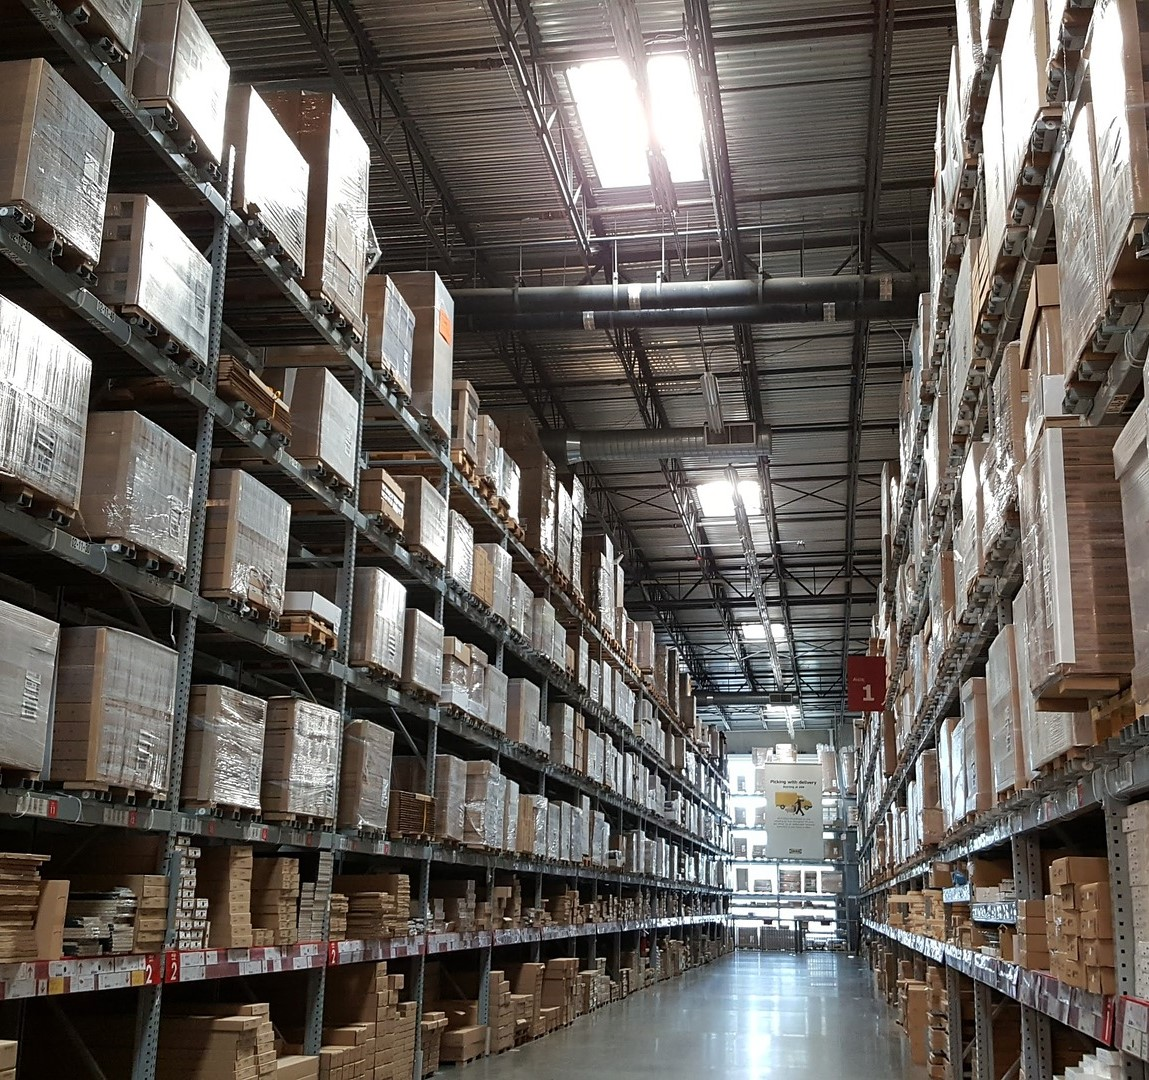
\includegraphics[width=0.5 \linewidth]{Images/store.jpeg}
\centering
\caption{A screen shot showing the predicted item details in the Bramhope store website}
\end{figure}
\newpage
\subsubsection{Tools Tab}
The Tools tab provides a function for calculating how many items are in a box.\\
There are three different fields that the user will have to complete. These are, the weight of the empty box, the weight of a single item as well as the weight of the filled bucket. From here, the number of items inside the box will be calculated and returned to the user.
\begin{figure}[H]
\includegraphics[width=0.4\linewidth]{Images/tools.jpeg}
\centering
\caption{A screen shot showing the Tools tab} 
\end{figure}

\pagebreak

\subsubsection{Contact us Tab}

This tab contains a form in which the users can fill in and send any queries or issues they have about the app.This can also be used by users to send a quotation request.The user must enter their name,email address and a query message as well as ticking the "Send location box" if the user would like to send their geo-location data.If the user would not like to send their location data, the user can deselect the send location box. 
\begin{figure}[H]
\includegraphics[width=0.5 \linewidth]{Images/contact.jpeg}
\centering
\caption{Contact Us Tab} 
\end{figure}

\subsubsection{Feedback page}

This section shows information about the development team and can be used for sending feedback or reporting any issues about the app to the Software Sharks development team. Reports can be bugs,errors and even suggestions on how to improve the app as a whole. 
\begin{figure}[!ht]
\includegraphics[width=0.4 \linewidth]{Images/feed.jpeg}
\centering
\caption{Feedback tab} 
\end{figure}
\newpage

%----------------------------------------------------------------------------------------
%	Using the System
%----------------------------------------------------------------------------------------
\pagebreak
\section{Using the System}
This section provides a detailed description of system functions. 
% This section forms the bulk of the user manual. It consists of a detailed description of the
% system functions. Each function (use case) should be described. Include screen captures
% and descriptive narrative to explain when, why and how each function is used.
% If the system has query or retrieval capabilities, the instructions necessary for recognition,
% preparation, and processing of a query applicable to a database should be explained in
% detail. If the system can create reports, describe all reports available to the end user.
% Include report format and the meaning of each field shown on the report.
% Use appropriate data examples to explain the full extent in which each function can be
% used.
\subsection{Using the Mobile app}

\subsubsection{Home tab}
This tab contains the main page of  the mobile app. The page contains a carousel of images and information on how to use the app. On opening of the app, this is the page that the user will be lead to.

\subsubsection{Submit an image}

\begin{enumerate}
\item Select Predict tab on the bottom navigation bar.(The tab with a Camera icon).
\item There are two options to select an image, Camera and Gallery. Choose one of these options.
\item For the camera option,the user must capture an image using the camera app that opens after clicking the camera option, after that the  user will be required to crop the image and save or discard it.
\item For the Gallery option, the Gallery app will open and the user can choose the picture they would like to identify, after that the  user will be required to crop the image and save or discard it.

\item Once the user has selected an image, click on the predict button in order to push the image to the image classification model.

\end{enumerate}

\subsubsection{Classification results}
\begin{enumerate}
\item Once the image has been pushed to the model, a prediction will be made and the results of this prediction will be displayed on the screen. The results will be displayed as a list with the name and accuracy percentage.
\item If the item is available in the Bramhope Catalogue, the user will be able to click the open icon on the side of the prediction name and result.This will send the user to an external website which has more information about how to purchase the item.
\end{enumerate}


\subsubsection{Tools tab}
The Tools tab is used to calculate the amount of items in a bin.\newline
N.B: The user has to use the same units (e.g grams) for each value for the function to output the correct results. 
\begin{enumerate}
\item The user will have weigh a single item from the box and input the result into the single item field.
\item The user will then have to weigh the empty bucket and input the result into the empty bucket field.
\item The final step will be for the user to input the weight of the filled bucket
\item After entering the weights,the system will automatically calculate the result and display it at the bottom of the screen
\end{enumerate}

\subsubsection{Contact us Tab}
The user can use this section to send quotes or any query of their choice (related to the products they would like to identify).
\newline
\begin{enumerate}
\item The user has to enter their name on the "Full name" field
\item The user has to enter their email address on the "Email address" field
\item The user has to enter their message on the "Message" field
\item The user can choose to tick the location box to send their location as well.This option is not required but rather recommended. 
\item Once all the fields have been completed, the user will have to select the "Send" button and a message to say that the message has sent will appear.
\end{enumerate}



\subsubsection{About us page}
This section displays information about the developers behind the mobile app and users can also send feedback or report issues to the Software Sharks Development team.

\subsection{Using the Web app}
\subsubsection{Home tab}
This tab contains the main page of the website. This shows the user how Ninshiki's image classification works. This is the page that the user will be lead to when entering the site into a web browser address bar.

\subsubsection{Submitting an image on the classify image page}

\begin{enumerate}
\item To submit an image, The  user must click on the classify image tab on the top navigation bar.
\item The user should now choose a method of selecting an image to be classified. The two options are taking a picture with the Webcam and File selection.
\item For the Webcam capture option, the user must capture an image using the Webcam on their computer (The user has to allow the browser use the Webcam).

\item If the user decides to choose the file select option,the file select interface will open and the user can choose the picture they would like to identify from their computer files. 

\item The user can also choose to use a general classifier or a Bramhope classifier (this classifier consist only Bramhope products). 

\item After a successful selection of a picture, the submit button will appear.The user should now click on the submit button to push the image to the image classification model.

\end{enumerate}

\subsubsection{Classification results}
\begin{enumerate}
\item After submitting the image the results will be displayed, with the name of the item  with the highest prediction percentage at the top.
\item The user can now click on the go to store link.(only if the item is available in the Bramhope Catalogue. This selection will send the user an external website which has more information about how to purchase the item.
\end{enumerate}


\subsubsection{Tools page}
The Tools tab is used to calculate the amount of items in a bin.\newline
N.B: The user has to use the same units (e.g grams) for each value for the function to get the correct results. 
\begin{enumerate}
\item The user will have weigh a single item from the box and input the result into the single item field.
\item The user will then have to weigh the empty bucket and input the result into the empty bucket field.
\item The final step will be for the user to input the weight of the filled bucket
\item After entering the weights,the system will automatically calculate the result and display it at the bottom of the screen
\end{enumerate}

\subsubsection{Contact us Page}
The user can use this section to send quotes or any query of their choice(related to the Bramhope products they want to identify).
\newline
\begin{enumerate}
\item The user has to enter their name on the "Enter your name" field
\item The user has to enter their email address on the "Enter your email address" field
\item The user has to enter their query on the "Enter your query" field
\item The user can now click submit to send the query to the Bramhope staff.
\end{enumerate}



\subsubsection{Feedback Footer}
This footer appears at the bottom of every page of the web sites. Users can use it to send feedback or report issues to the Software Sharks Development team. Users can choose the type of feedback,the options can be chosen from a drop down menu,the options are General Feedback, Bug and Feature reports.






\pagebreak

%----------------------------------------------------------------------------------------
%	Troubleshooting
%----------------------------------------------------------------------------------------
\section{Troubleshooting}
% Describe all recovery and error correction procedures, including error conditions that may
% be generated and corrective actions that may need to be taken.
% If there are special actions the user must take to insure that data is properly saved or
% that some other function executes properly, describe those actions here. Include screen
% captures and descriptive narratives, if applicable. For example, Show screen shots of error
% messages produced by your system and for each explain what may have caused the error
% and explain how the user can avoid the error.
The following errors may occur:
\subsection{GPS Coordinates not found}
This error occurs when the user tries to send a query in the contact us tab(with the send location box ticked)  while the GPS of the device is turned off.
\newline
To recover from this error the user must turn on the the GPS on their device settings and resend the query again.
\subsection{AI computation Error}
This Error happens to Mobile phones that do not support AI computations when the user try to click on the predict button to upload an image.
The user must use an AI computation supporting device to prevent this error.

\subsection{Error getting selected Image}
This error Occurs when the user clicks on the camera/gallery button and selects back without choosing an image 
\newline
To recover from this error,the user should press "Ok" and re-select the picture by pressing the camera or gallery  button again.

\subsection{Lagging/slow web app}
Laggy/slow web app - This error occurs when the browser running the web app lacks the required WebGL version for image prediction calculations.The website will be very slow will not be usable.
\newline
This can be resolved by using a compatible browser and ensuring that the system is able to run WebGL such as Google Chrome, Firefox, Safari, and Opera.

\end{document}